%\chapter{Preliminaries}



\chapter{提案手法}

\section{問題設定}

そのような問題点を踏まえ,提案手法では複数の参照点を学習に利用する手法を導入した.従来手法の拡張で複数の参照点を考慮できるようにするためには,参照点と変位(座標系)のいずれかに複数の参照点の情報を保持する機構を導入する必要がある.そこで参照点の候補に各参照点間の重心位置を採用することによって,参照点に複数の参照点の位置情報を含めることができると考えた.また本研究では物体移動動作を初期状態に対する最終状態の決定と定義し,動作中のトラジェクタ軌跡に関しては考えていないため,学習モデルはより単純なガウスモデルを使用した.
重心位置を参照点として考慮した際,構成する参照点同士の位置関係に対応した相対位置を学習するために,重心位置を原点として重心を構成する参照点の向きに軸を取る座標系を考慮する必要がある.そのため,重心位置に対する変位にはその構成参照点の数分の座標系を追加生成する.

\section{提案手法の概要}

\subsection{参照点}

従来手法で採用されていた各物体位置,トラジェクタの初期位置,画面中央に加えて,提案手法では新たに2つ以上の任意の物体間の重心位置を参照点に含める.すなわち環境中の$n$個の物体に対して,参照点は$2^{n}$個考慮する.

\subsection{変位}

従来手法で考慮されていた2つの変位に加えて,複数の物体を考慮した動作の学習を実現するために提案手法では以下の3種類が存在するとする.

	\begin{enumerate}
		\item 参照点を原点とし,常に一定の相対位置に遷移する
		\item 参照点を原点とし,トラジェクタの初期位置に応じて遷移先が変化する
		\item 複数の物体の位置関係に応じて遷移先が変化する
	\end{enumerate}
これら3種類の違いについてFig.\ref{figure:difference_displacement}で示す.以下,本文中ではFig.\ref{subfigure:difference_displacement1}を恒等座標$k_{id}$,Fig.\ref{subfigure:difference_displacement2}をランドマーク-トラジェクタ座標$k_{lt}$,Fig.\ref{subfigure:difference_displacement3}を重心-ランドマーク座標$k_{gl}$と定義する.

		%%%%%%%%%%%%%%%%%%%%%%%%%%%%%%%%%%%%%%%%%%%%%%%%%%%%%%%%%%%%%%%%%%%%%%%%%%%%%%%%%%%%%%%%%%%%%%%%%%%%%%%
		%	\begin{figure}[t]
		%中央ぞろえ
		%		\begin{center}
		%			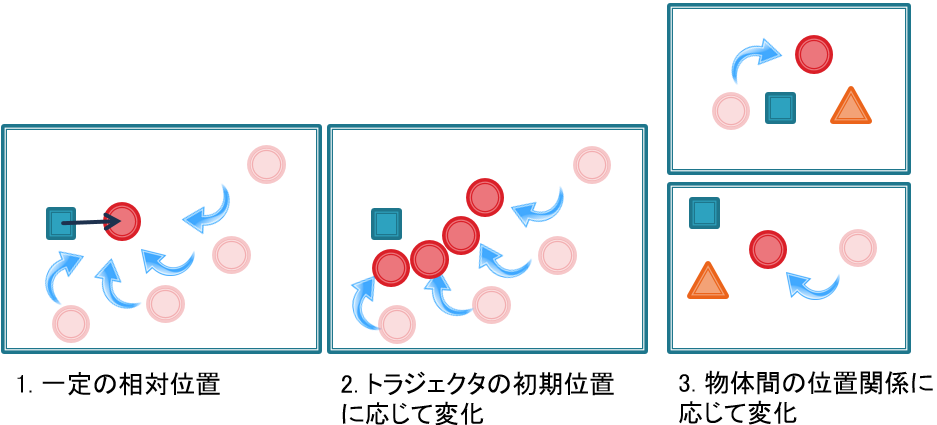
\includegraphics[width=14cm]{figure2.png} \\ %Teの基本として, \\ で緊急改行ができる.(今回の場合や行列などを除き,あまり使わない)
		%			\caption{参照点に対する遷移の違い}
		%			\label{figure:difference_displacement}
		%		\end{center}
		%	\end{figure}
		%%%%%%%%%%%%%%%%%%%%%%%%%%%%%%%%%%%%%%%%%%%%%%%%%%%%%%%%%%%%%%%%%%%%%%%%%%%%%%%%%%%%%%%%%%%%%%%%%%%%%%%

%%%%%%%%%%%%%%%%%%%%%%%%%%%%%%%%%%%%%%%%%%%%%%%%%%%%%%%%%%%%%%%%%%%%%%%%%%%%%%%%%%%%%%%%%%%%%%%%%%%%%%%
\begin{figure}[h]
	\centering
	\begin{minipage}[t]{.3\textwidth}
		\centering
		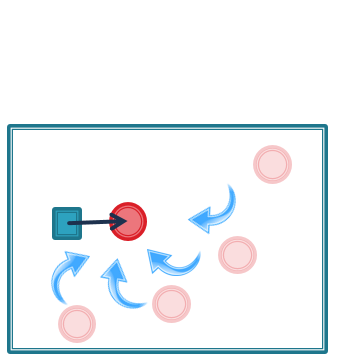
\includegraphics[width=4.7cm]{figure2_sub_a.png} \\ %TeXの基本として, \\ で緊急改行ができる.(今回の場合や行列などを除き,あまり使わない)
		\subcaption{トラジェクタ初期位置に対して一定}
		\label{subfigure:difference_displacement1}    
	\end{minipage}
	\begin{minipage}[t]{.3\textwidth}
		\centering
		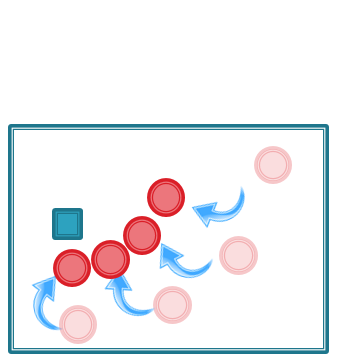
\includegraphics[width=4.7cm]{figure2_sub_b.png} \\ %TeXの基本として, \\ で緊急改行ができる.(今回の場合や行列などを除き,あまり使わない)
		\subcaption{空間上の特定の位置}
		\label{subfigure:difference_displacement2}
	\end{minipage}
	\begin{minipage}[t]{.3\textwidth}
		\centering
		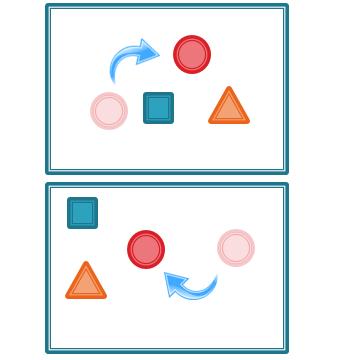
\includegraphics[width=4.7cm]{figure2_sub_c.png} \\ %TeXの基本として, \\ で緊急改行ができる.(今回の場合や行列などを除き,あまり使わない)
		\subcaption{他物体の位置に応じて変化}
		\label{subfigure:difference_displacement3}
	\end{minipage}
	\caption{参照点に対する遷移の違い}
	\label{figure:difference_displacement}
\end{figure}
%%%%%%%%%%%%%%%%%%%%%%%%%%%%%%%%%%%%%%%%%%%%%%%%%%%%%%%%%%%%%%%%%%%%%%%%%%%%%%%%%%%%%%%%%%%%%%%%%%%%%%%


Fig.\ref{subfigure:difference_displacement3}の例として,トラジェクタをある物体とある物体の間に動かすという動作などが挙げられる.
推定すべき観点は$2^{n}$個の参照点$l∈L$と3つの座標系$k∈K$の対として表される.以下,参照点$l$,座標系$k$の観点を$<l , k> ∈ V$と表すこととする.各観点$<l , k>$は確率モデルであるガウスモデルを持ち,その平均,2乗平均,標準偏差をそれぞれ$μ_{lk}$,$Q_{lk}$,$σ_{lk}$とする.

\section{動作学習}

与えられた教示動作から,以下のように各観点のガウスモデルを学習する.

\begin{equation}
	v = Normalize_{lk}(Transform_{lk}(p))
\end{equation}

\begin{equation}
	μ_{lk}  \leftarrow \frac{N}{N+1}μ_{lk}+\frac{1}{N+1}v
\end{equation}
\begin{equation}
	Q_{lk}  \leftarrow \frac{N}{N+1}Q_{lk}+\frac{1}{N+1}v^2	
\end{equation}
\begin{equation}
	σ_{lk}  \leftarrow \sqrt{Q_{lk} - μ_{lk}^2}
\end{equation}

ここで,$p$は教示動作の目標位置を指す.$Normalize_{lk}$,$Transform_{lk}$はそれぞれその観点における正規化関数と座標変換を指し,以下の式で与えられる.

%まず教示動作の目標位置の,各参照点を原点とした相対位置を求め,各座標系ごとに座標変換,正規化を行う.それにより得たベクトル$v$を用いて,観点$<l , k>$のガウスモデルの平均$μ_{lk}$,2乗平均$Q_{lk}$,標準偏差$σ_{lk}$をそれぞれ更新する.
\begin{equation}
	Transform_{lk}(v) = 
	\begin{pmatrix}
        	\cos θ_{lkv} & \sin θ_{lkv} \\
        	-\sin θ_{lkv} & \cos θ_{lkv}
	\end{pmatrix}
	(v-Position(l))
\end{equation}
\begin{equation}
	\label{equation:normalize}
	Normalize_{lk}(v) = 
	\begin{cases}
		v & (if\,\,k=k_{id}) \\
		\frac{unit}{| Position(L_{k})-Position(l) |}v & (otherwise)
	\end{cases}
\end{equation}

ただし,$unit$は正規化長を表し,

\[
	\cos θ_{lkv} = \frac{(v-Position(l))・(Position(L_{k})-Position(l))}{| v-Position(l) || Position(L_{k})-Position(l) |}
\]

であり,$Position(l)$は参照点$l$の位置ベクトルを表す.また$L_{k}$は座標系$k$に特有の参照点を表す.例えば座標系$k_{lt}$の場合,$L_{k_{lt}}$はトラジェクタの初期位置を表す.
正規化関数の必要性と性質については\ref{subsection:UNIT}で述べる.

動作学習のアルゴリズムの詳細については付録\ref{appendix3}に示す.

\section{動作再現}

教示動作から学習された各観点$<l , k>$における確率モデルを用いて,トラジェクタの目標位置$v$を以下のように求めることで,学習動作の再現を行う.
\begin{equation}
	v =  Position(\hat{l}) +Transform^{-1}(Normalize^{-1}(μ_{\hat{l}\hat{k}})) 
\end{equation}
\begin{equation}
	<\hat{l} , \hat{k}> =  \mathop{\arg\min}_{k , l}σ_{lk}
\end{equation}

まず学習された各観点のガウスモデルのうち,最も分散の小さいものを探索する.分散が小さいとは教示動作がその観点に対して常に類似した目標位置に遷移していたことを意味し,教示者が意図した観点である可能性が高いと考えられるためである.選択された観点のガウスモデルの平均を,その観点と再現時の初期環境に応じた正規化と座標変換の逆関数を計算し,初期環境における参照点の位置に平行移動することで再現動作のトラジェクタの目標位置を推定する.
Fig.\ref{figure:learning_and_reproduction_model}に,提案手法における動作学習と動作再現の模式図を示す.
また付録\ref{appendix3}に,動作再現のアルゴリズムの詳細を示す.
%%%%%%%%%%%%%%%%%%%%%%%%%%%%%%%%%%%%%%%%%%%%%%%%%%%%%%%%%%%%%%%%%%%%%%%%%%%%%%%%%%%%%%%%%%%%%%%%%%%%%%%
	\begin{figure}[h]
%中央ぞろえ
		\begin{center}
			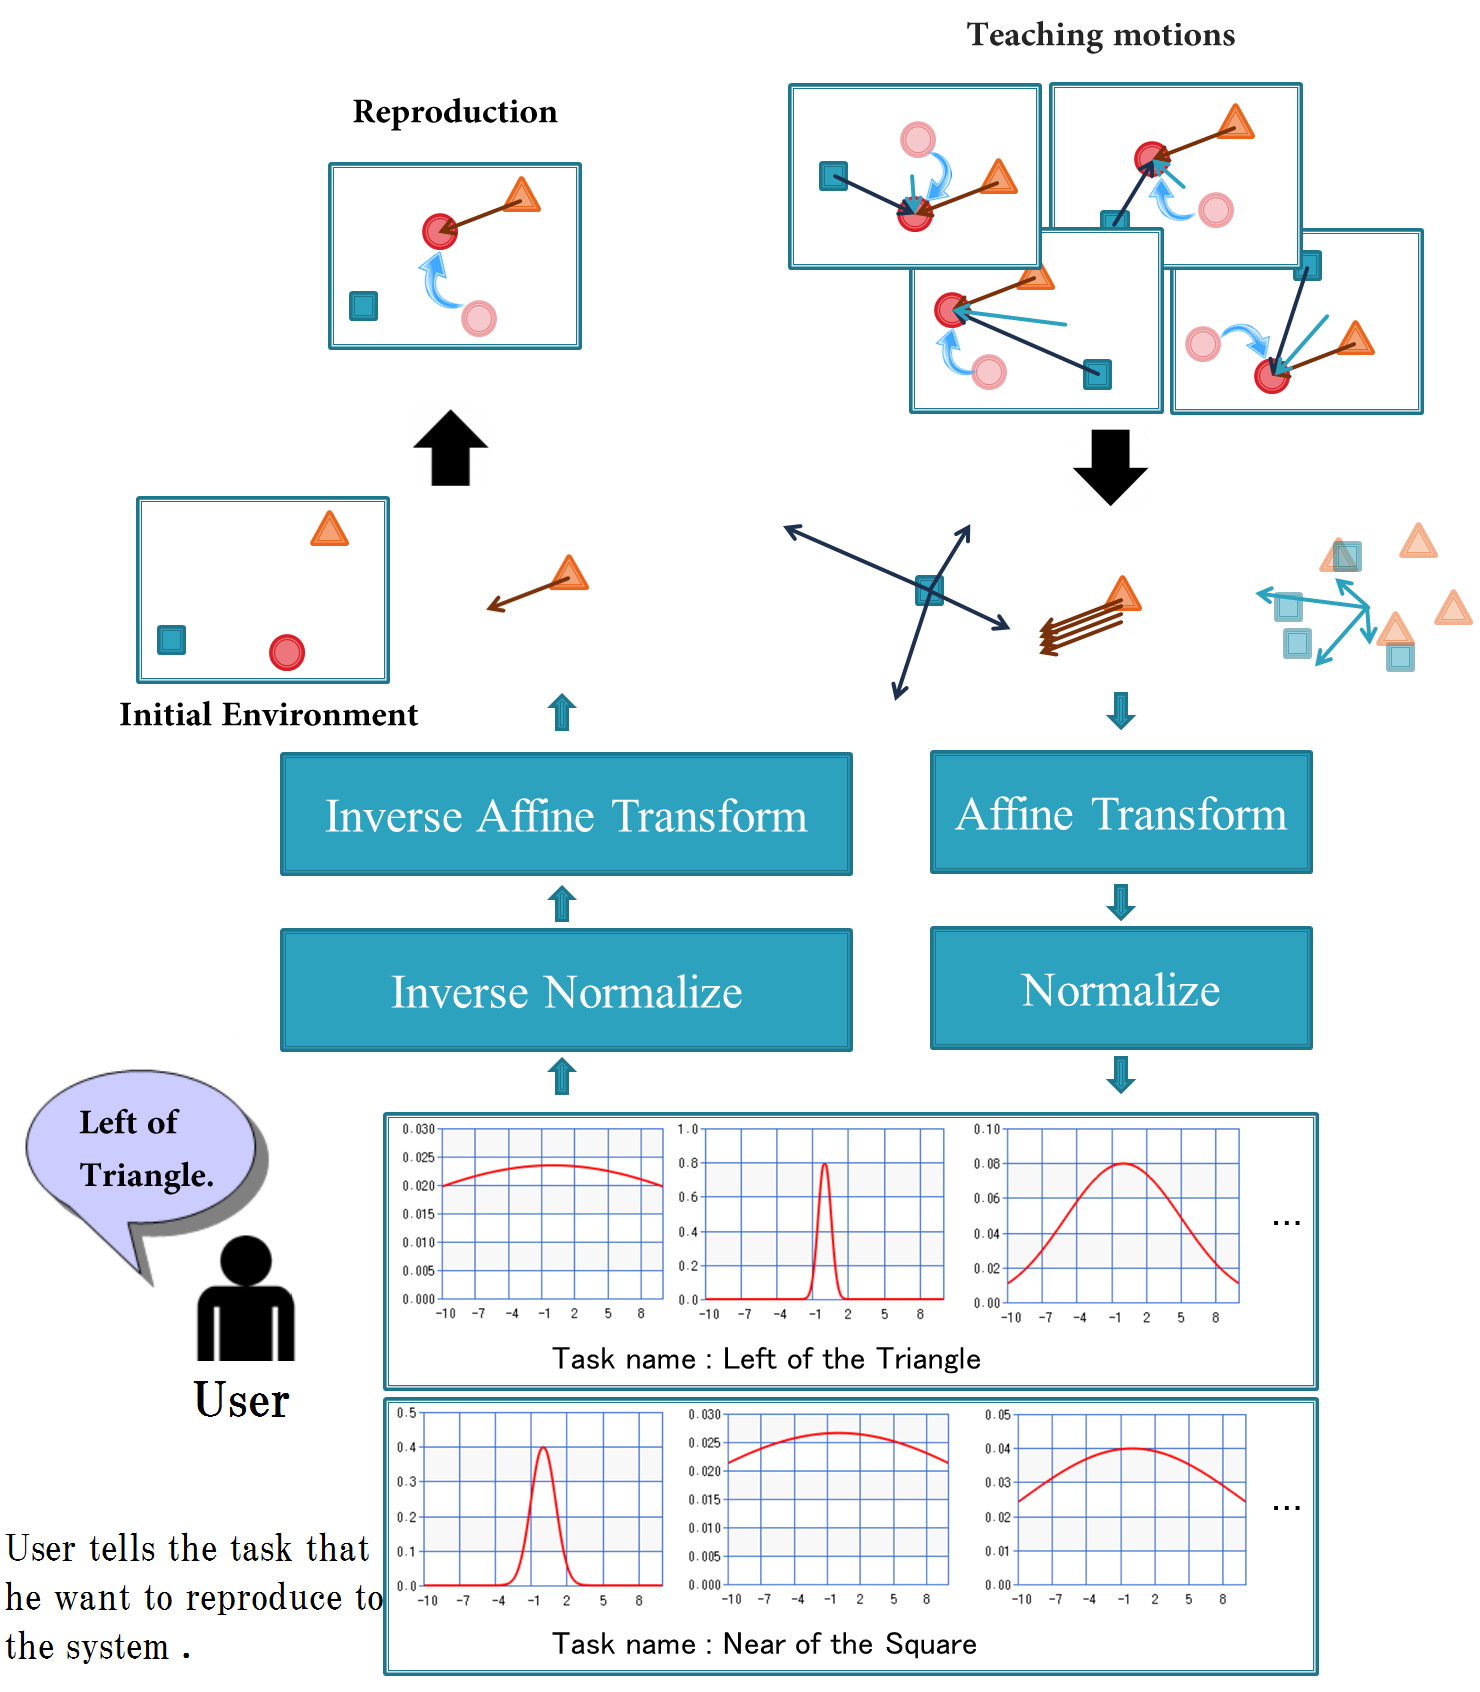
\includegraphics[width=12cm]{chart9.png} \\ %Teの基本として, \\ で緊急改行ができる.(今回の場合や行列などを除き,あまり使わない)
			\caption{動作学習と動作再現}
			\label{figure:learning_and_reproduction_model}
		\end{center}
	\end{figure}
%%%%%%%%%%%%%%%%%%%%%%%%%%%%%%%%%%%%%%%%%%%%%%%%%%%%%%%%%%%%%%%%%%%%%%%%%%%%%%%%%%%%%%%%%%%%%%%%%%%%%%%

\section{動作識別}

動作ごとに学習された観点集合$V_{t}$を用いて,目標位置が$p$である例示動作の属する動作$t∈T$を以下のように推定することで,例示動作の識別を行う.

\begin{equation}
	\label{equation:identification function}
	t =  \mathop{\arg\max}_{t}Probability(<l , k>∈V_{t} , p)
\end{equation}

\begin{equation}
	\label{equation:generation probability}
	Probability(<l , k> , p) = \frac{1}{\sqrt{2\pi}σ_{lk}}\exp \left(\frac{|Normalize_{lk}(Transform_{lk}(p))-μ_{lk}|^2}{2σ_{lk}^2}\right)
\end{equation}

ここで$T$は既学習動作集合を表し,$V_{t}$とは動作$t$を学習した観点の集合を表す.
まず各動作において学習されたガウスモデルから,$p$が生起される確率である\ref{equation:generation probability}式をそれぞれ求め,生起確率が最大となるガウスモデルを持つ動作を識別結果とする.また,\ref{equation:identification function}式に閾値を設定し,以下のように定義し直すことで,未学習動作の推定が可能になる.

\begin{equation}
	\label{equation:identification function2}
	t =
	\begin{cases}
		\mathop{\arg\max}_{t}Probability(V_{t} , p)		& (\mathop{\max}_{t}Probability(V_{t} , p) > Threshold) \\
		t_{unknown}					 			& (otherwise)
	\end{cases}	
\end{equation}
ここで,$t_{unknown}$は未学習動作を表す.
付録\ref{appendix3}に,動作識別のアルゴリズムの詳細を示す.


%Fig.\ref{figure:identification_model}に,提案手法における動作識別の模式図を示す.
%%%%%%%%%%%%%%%%%%%%%%%%%%%%%%%%%%%%%%%%%%%%%%%%%%%%%%%%%%%%%%%%%%%%%%%%%%%%%%%%%%%%%%%%%%%%%%%%%%%%%%%
%	\begin{figure}[h]
%中央ぞろえ
%		\begin{center}
%			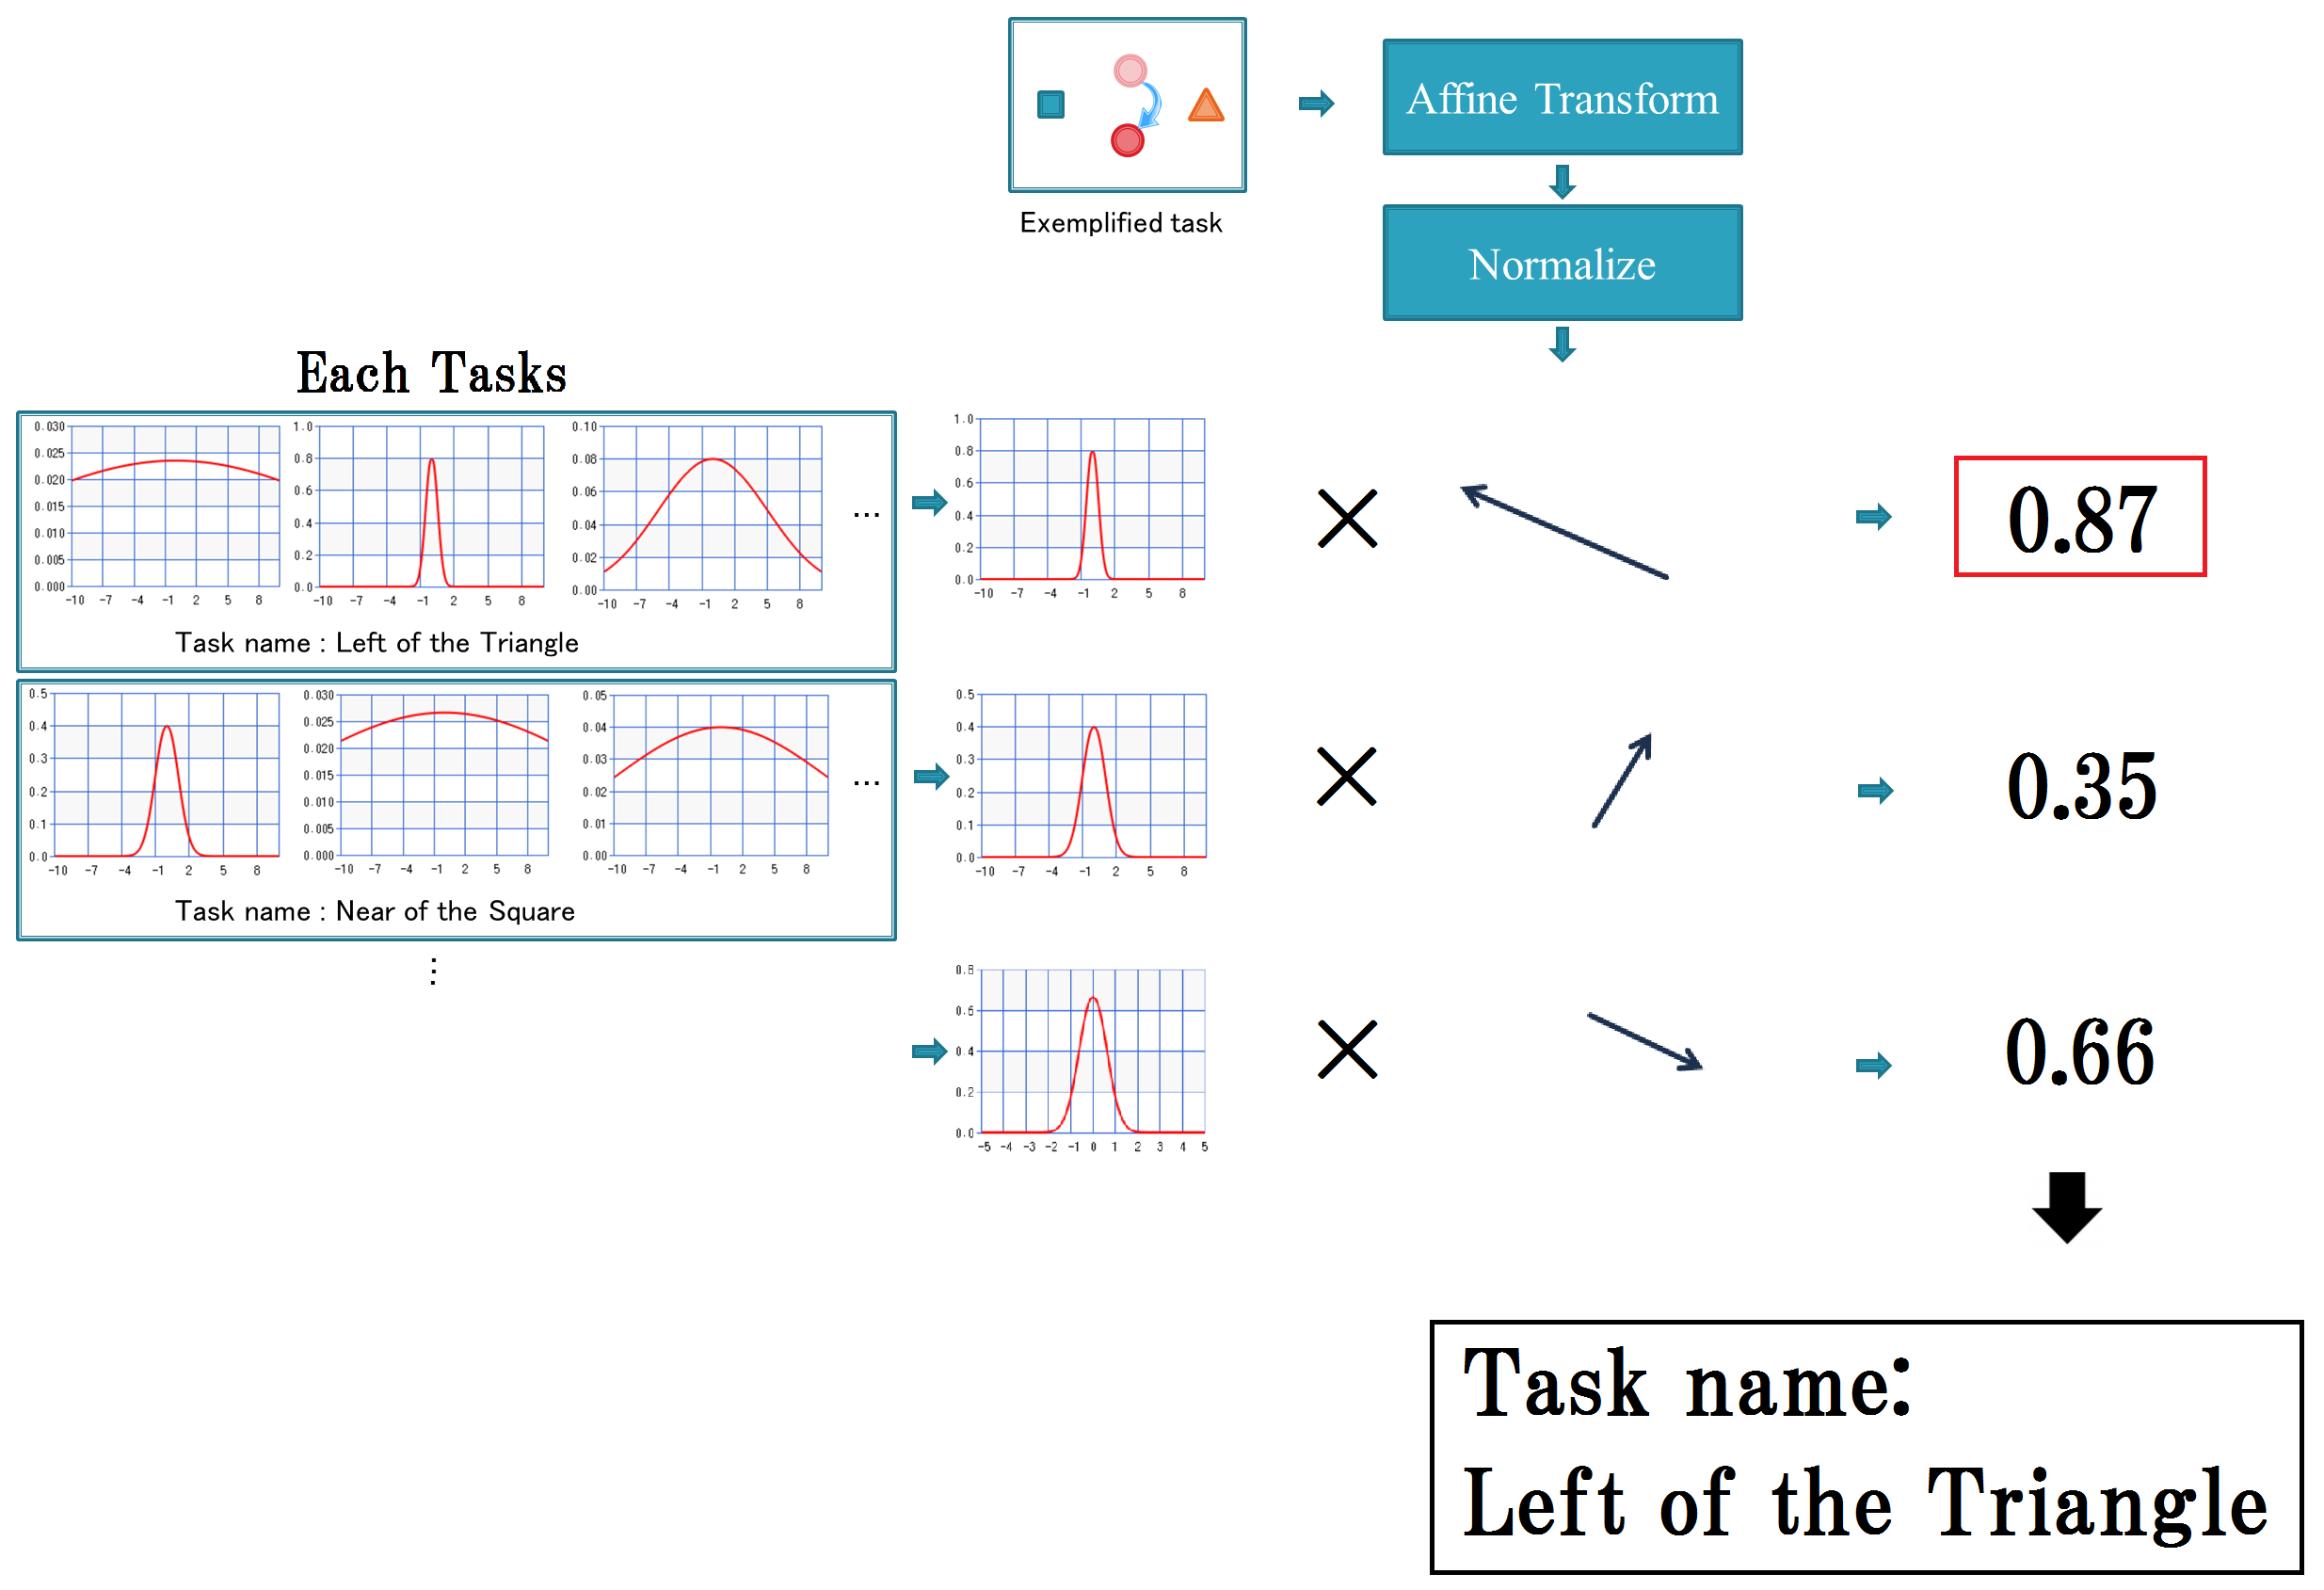
\includegraphics[width=14cm]{chart10.png} \\ %Teの基本として, \\ で緊急改行ができる.(今回の場合や行列などを除き,あまり使わない)
%			\caption{動作識別}
%			\label{figure:identification_model}
%		\end{center}
%	\end{figure}
%%%%%%%%%%%%%%%%%%%%%%%%%%%%%%%%%%%%%%%%%%%%%%%%%%%%%%%%%%%%%%%%%%%%%%%%%%%%%%%%%%%%%%%%%%%%%%%%%%%%%%%
